\documentclass[a4paper,10pt,twocolumn]{article}
\usepackage[T1]{fontenc}
\usepackage[utf8]{inputenc}
\usepackage{lmodern}
\usepackage[francais]{babel}
\usepackage{textcomp}
\usepackage[top=2cm,bottom=2cm,left=2cm,right=2cm]{geometry}
\usepackage{amsmath}
\usepackage{amssymb}
\usepackage{mathrsfs}
\usepackage{float}
\usepackage{icomma}
\usepackage{gensymb}
\usepackage{graphicx}
\usepackage[font=sf, labelfont={sf,bf}, margin=1cm]{caption}
\usepackage[french,onelanguage,ruled,lined]{algorithm2e} % pour pseudo code
\usepackage{array}

\title{\huge \textbf{Technique pour l'extraction de plaque d'immatriculation}}
\author{Alexandre \bsc{Bonhomme} - \small{BONA20128906}}
\date{\today}

\begin{document}

\maketitle

\section{Introduction}
L'identification automatique de plaque d'immatriculation (Automatique Licence Plate Identification : ALPI) est une des étape indispensable dans la gestion automatique du traffic routier. Elle peut par exemple être utilisé pour l'indentification de véhicules en infractions sur l'autoroute ou en complément des radars automatiques.\\
Les algorithme de d'itentification automatique peuvent se décomposer en deux parties : 
\begin{enumerate}
  \item Détection et extraction de la plaque d'immatriculation
  \item Reconnaissance des caractères
\end{enumerate}
Mon travail traite uniquement de la première partie et repose essentiellement sur un article, de Chirag N. Paunwala et Suprava Patnaik\cite{paunwala10}, qui présente une technique simple et efficace d'extraction d'une ou plusieurs plaques d'immatriculation dans différentes conditions.

\section{Présentation de l'algorithme}
N'ayant pas implémenté toutes les parties de l'algorithme proposé je ne détaillerais pas celle-ci dans ce rapport. J'ai de plus apporté quelques modification personnel que j'expliquerai par la suite.

\subsection{Prétraitement}
La majorité des traitements effectués, dans l'algorithme proposé, travaillent sur des images en niveaux de gris. Il faut donc appliquer une convertion depuis les images sources RGB. Pour cela la formule suivante à été utilisée :
\begin{gather}
  I(i, j) = 0.114\times R(i, j) + 0.587\times G(i, j) {} \\ {} + 0.299\times B(i, j)\nonumber
\end{gather}
avec $I(i,j)$ la valeur en niveaux de gris, et $R(i,j), G(i,j) \text{ et } B(i,j)$ respectivement les valeurs des niveau de rouge, vert et bleu.

\subsection{Analyse des contours verticaux}
L'étentiel de cette algorithme ce base sur des connaissances à prioris que nous avons sur l'image. En l'occurence, une plaque s'immatricution standards comporte de nombreuse discontinuités verticales dues à la présence de caractère noirs sur un fond blanc ou jaunes.

Pour tenter de localiser la position de la plaque il apparait dons intéressant d'effectuer une recherche dans contour verticaux. Pour cela il est proposé de calculer le gradient verticale de l'image :
\begin{align}
  G_v(i, j) = |I(i, j + 1) + I(i, j)|
\end{align}
\begin{figure}[H]
	\centering 
	  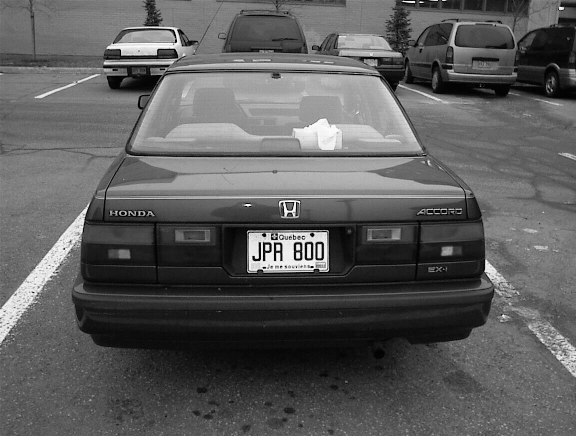
\includegraphics[width=100pt]{img/991213-006.png}
	  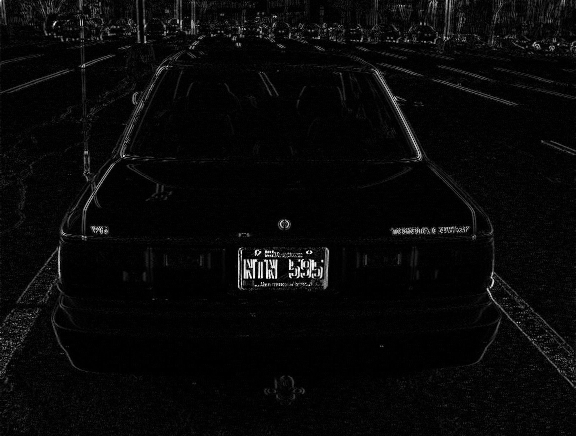
\includegraphics[width=100pt]{img/991213-006_grad.png}
	\caption{Image d'origine et Image de son gradient verticale\label{grad}}
\end{figure}

\subsection{Projection horizontale et filtrage Gaussien}
Comme le montre la Figure~\ref{grad} on a des valeurs de gradient très élevé au niveau de la location de la plaque d'immatriculation. En partant de ce principe les auteurs de l'article propose d'effectuer une projection horizontale (\ref{eq:proj_h}) et de ne garder que les bandes de l'image ou la projection est supérieur à un certain seuil.
\begin{align} \label{eq:proj_h}
  P_h(i) = \sum_{j=1}^{n}G_v(i, j)
\end{align}
Cependant, comme le montre la Figure~\ref{h_proj_gauss}, la projection horizontale est très bruitée. Pour résoudre se problème les auteurs de l'articles propose d'appliquer le filtrage Gaussien décrit en (\ref{eq:filter_gauss_1}).
\begin{gather} \label{eq:filter_gauss_1}
  P_h(i)^{\prime} = \frac{1}{2 \sum_{j = 1}^{w} h(j, \sigma) + 1} \times\\ 
  \left[ P_h(i) + \sum_{j = 1}^{w} P_h(i - j)h(j, \sigma) + P_h(i + j)h(j, \sigma) \right]\nonumber
\end{gather}
avec 
\[ h(j, \sigma) = e^{\frac{-j\sigma^2}{2}} \]
Les paramètres $w$ et $\sigma$ on été déterminés de manière empirique et les valeurs retenues sont $w = 6$ et $\sigma = 0.05$.

Grâce à cette technique on réduit considérablement le temps de calcule en limitant les zones de recherches comme le montre la Figure~\ref{v_filter}.
\begin{figure}[H]
	\centering 
	  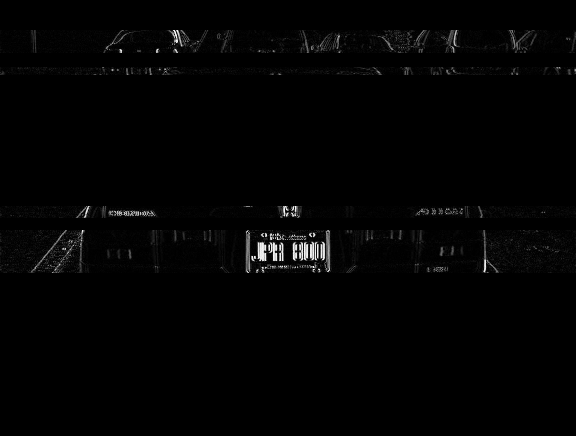
\includegraphics[width=200pt]{img/991213-006_v_filter_1-2.png}
	\caption{Gradient verticale après un premier filtrage\label{v_filter}}
\end{figure}
En partant d'une constation simple j'ai réussis à réduire d'avantage les zones de recherches. En effet, il est quasiment impossible qu'une plaque d'immatriculation se situe dans la partie haute de l'image celle si ce situant généralement dans la partie basse. J'ai donc appliqué un second filtrage Gaussien qui favorise la zone du bas de l'image:
\begin{equation}
  P_h^{\prime\prime}(i) = P_h^{\prime}(i) \times e^{\frac{(i - \mu)^2}{2\sigma^2}}
\end{equation}
avec 
\begin{align*}
  \mu & = H - H\times \frac{5}{2}\\
  \sigma & = \frac{H}{3}
\end{align*}
$H$ étant la hauteur de l'image (donc la taille du vecteur de projection).

\begin{figure}[H]
	\centering 
	  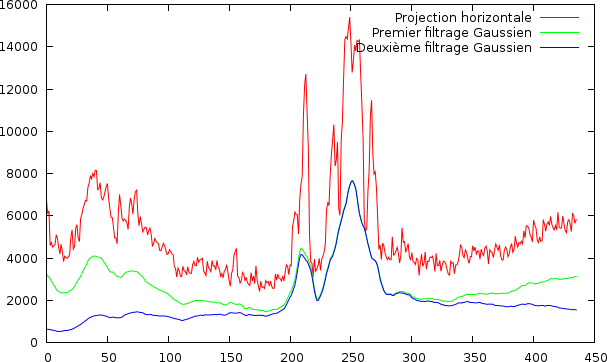
\includegraphics[width=210pt]{img/project_h_gauss.png}
	\caption{Projection horizontale et filtrage Gaussien\label{h_proj_gauss}}
\end{figure}

Comme on peut l'observer sur la Figure~\ref{v_filter_gauss} cela réduit encore l'ensemble en supprimant des zones précédement conservées par le premier filtrage tout en conservant les zones basses de l'image.
\begin{figure}[H]
	\centering 
	  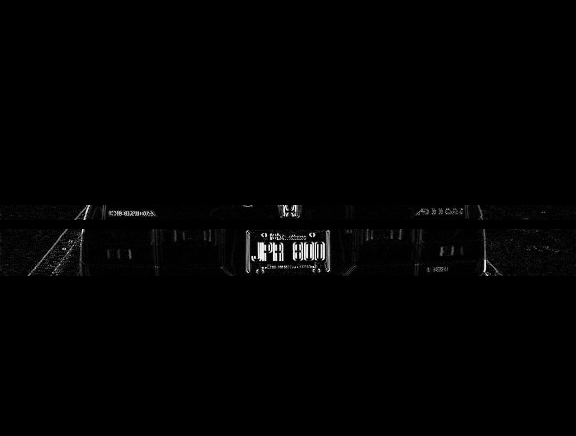
\includegraphics[width=200pt]{img/991213-006_v_filter_gauss.png}
	\caption{Gradient verticale après le second filtrage\label{v_filter_gauss}}
\end{figure}

Le seuil (\ref{eq:seuil_1}) utilisé pour le filtrage $T$ est une pondération de la moyenne des projection $m$ par un coéfficient $w_t \in [1.2, 1.4]$. La valeur du coéfficient utilisé dans l'article est de $1.2$, mais suivant la nature de l'image on obtient de plus ou moins bon résultats avec un coéfficient légèrement plus élevé.
\begin{equation} \label{eq:seuil_1} 
  T = w_t \times m
\end{equation}

\subsection{Détection des composantes connexes}
Afin de pouvoir détecter les composantes connexes il faut préalablement traiter le résultat du gradient avec différente opérateur morphologique tel que l'ouverture et la fermeture. L'opération d'ouverture correspond à l'application succéssive d'un masque d'érosion et d'un masque de dilatation de même taille. La fermeture quant à elle s'effectue en appliquand d'abord un masque de dilatation puis un masque d'érosion. L'ouverture permet de supprimer les composantes isolées et la fermeture permet de combler les "trous" au sein des zones connexes.

Ces opérations requièrent une binarisation de l'image qui à été effectuée grâce à un seuillage par histogramme légèrement modifié pour ne pas tenir compte des niveaux de gris égaux à 0.
\begin{figure}[H]
	\centering 
	  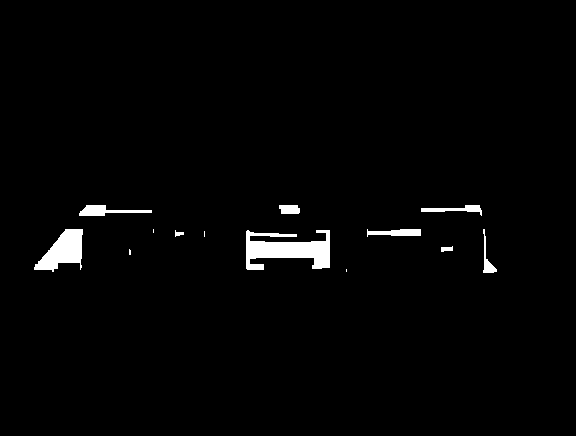
\includegraphics[width=200pt]{img/991213-006_morpho.png}
	\caption{Application des opérateurs morphologiques\label{morpho}}
\end{figure}
Le résultats présenté dans la Figure~\ref{morpho} à été obtenu en appliquant successifs le masque de fermeture (\ref{eq:closing}) (de taille $20 \times 3$) et le masque d'ouverture (\ref{eq:opening}) (de taille $1 \times 5$).
\begin{gather}
  \label{eq:closing}
  \left( \begin{array}{c} 
    1 1 1 1 1 1 1 1 1 1 1 1 1 1 1 1 1 1 1 1\\
    1 1 1 1 1 1 1 1 1 1 1 1 1 1 1 1 1 1 1 1\\
    1 1 1 1 1 1 1 1 1 1 1 1 1 1 1 1 1 1 1 1    
  \end{array} \right)\\
  \label{eq:opening}
  \left( \begin{array}{c} 
    1\\
    1\\
    1\\
    1\\
    1   
  \end{array} \right)
\end{gather}

Une fois ces traitements effectués un algorithme de recherche des composantes connexes à été appliqué.
\begin{figure}[H]
	\centering 
	  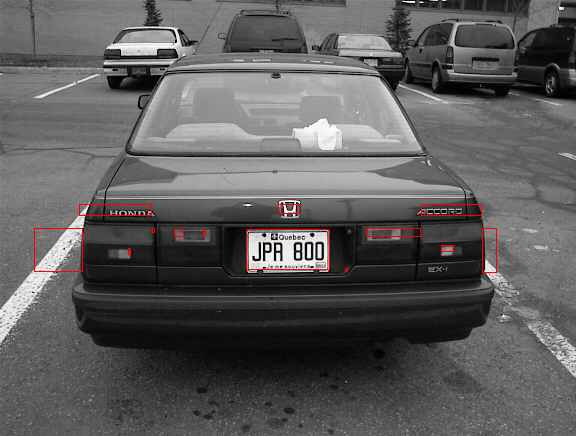
\includegraphics[width=200pt]{img/991213-006_detect_1.png}
	\caption{Localisation des composantes connexes\label{connexes}}
\end{figure}

\subsection{Filtrage des zones détectées}
Afin d'éliminter une grande partie des zones détectées par l'algorithme de recherche les auteurs proposent de tenir compte de la morphologie d'une plaque d'immatriculation tel que la hauteur, la largeur et le ratio hauteur/largeur.

\subsubsection{Analyser de la rectangularité et du ratio} 
Pour effectuer cette analyse nous partons de connaissances à prioris sur les plaques d'immatriculations. Nous savons qu'une plaque réglementaire doit avoir un aspect plus ou moins restangulaire. Ainsi son ratio devrait être comprit entre 0,2 et 0,7. On fixera, en plus de cela, une longueur et une largeur minimale/maximale qui pourront être adaptés suivant le contexte d'utilisation. Les valeurs que j'ai retenu sont légèrement différentes de l'article originale (qui traite exclusivement des plaques Indiennes). Les plaque considérées comme potentiellement admissibles devront avoir une largeur et une hauteur minimum respectivement de 35 et 7; et une largeur et une hauteur maximum de 200 et 60.
\begin{figure}[H]
	\centering 
	  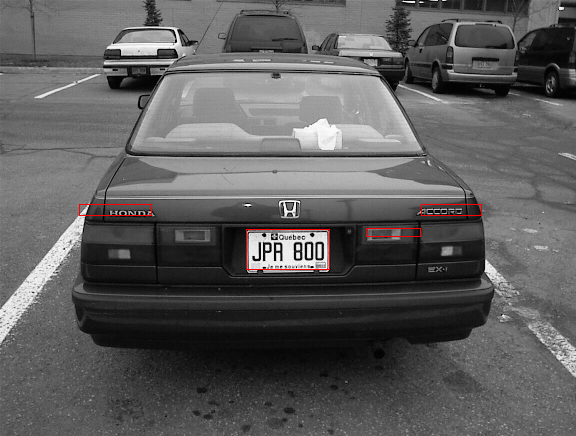
\includegraphics[width=200pt]{img/991213-006_detect_2.png}
	\caption{Localisation des composantes connexes après filtrage\label{connexes_2}}
\end{figure}
Comme le montre la Figure~\ref{connexes_2} ce filtrage réduit considérablement les zones de recherches, mais certaines zones de "non plaque" restent tout de même détectées.

\subsubsection{Detection de contours}
Suite à un seuillage automatique utilisant la technique de Ostu\cite{otsu79} un processus d'érosion (\ref{eq:erode}) et de dilatation (\ref{eq:dilate}) est réalisé pour tenter améliorer les contours dans la zone de detection.
\begin{gather}
  \label{eq:erode}
  \left( \begin{array}{c} 
    1 1\\
    1 1
  \end{array} \right)\\
  \label{eq:dilate}
  \left( \begin{array}{c} 
    1\\
    1\\
    1 
  \end{array} \right)
\end{gather}

\subsubsection{Analyse des points d'intérêts}
Le dernier filtrage effectué permet didentifier, parmis les zones retenues, les plaques d'immatriculations valides. Pour cela les l'auteurs de l'article proposent de mesurer les variations présente entre les caractères de la plaque et sont arrière plan. Les mesures sont effectuées horizontalement à trois endroits clées de chaque zones :
\begin{align*}
  \frac{H}{3}, \frac{H}{2}\text{ et }H - \frac{H}{3}
\end{align*}
avec $H$ la hauteur de la zones (cf. Figure~\ref{plate_bin}).
\begin{figure}[H]
	\centering 
	  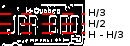
\includegraphics{img/plate_bin.png}
	\caption{Mesure des variations verticales au sein d'une zone\label{plate_bin}}
\end{figure}
La technique proposée fonctionne relativement bien et permet d'éliminer la majorité des faux positifs. Cependant celle-ci comporte plusieurs problèmes. En effet, si l'on mesure indépendamment les variations des trois zones celle-ci est très sensible au bruit de type "poivre et sel" (généré par la binarisation de zones bruitées). Une solution serait alors de mesurer simultanément les variations aux trois endroits. Cette solution est tout à fait viable pour les plaques parfaitement horizontales mais devient beaucoup moins efficase lors d'une légère inclinaison de la plaque (déformation du à la perspective par exemple). 

Afin de tenter de résoudre ce problème j'ai mis en place une pondération de la mesure de variation de tel sorte qu'une changement d'état simultané des trois zones apporte une contribution plus forte qu'une variation de deux zones ou que'une unique variation. Les poids qui sont apparues les plus naturels sont $2, 1 \text{ et } 0.5$.

L'algoritme initial propose ensuite d'effectuer un seuillage simple afin de ne garder que les zones possédant un nombre de variations suffisantes. Lors de l'implémentation de cette technique j'ai pu constater que le nombre de variations verticales correspondant à une plaque est relativement dépendant de la taille de la zone (la cause étant la taille du masque utilisé lors de l'érosion/dilatation appliqué lors de la détection de contours). J'ai donc mis en place un clacul du ratio de variation
\begin{equation}
  R_v = \frac{v}{H+L}
\end{equation}
avec $H \text{ et } L$ respectivement la hauteur et la largeur de la zone, et $v$ le nombre de variations précédement mesurées.

Un double seuillage (cf. Algorithme~\ref{seuil_2}) est alors effectué semblable à un seuillage par hystérésis.
\begin{algorithm} 
	\caption{Seuillage varation\label{seuil_2}}
	\KwIn{$v, R_v$}
	
	\If{($v > T_b$ et $v < T_h$ et $R_v > Tr_b$) ou ($R_v > Tr_h$)}{
	  {\tt ConserverZone()}\;
	}
\end{algorithm}\\
Après expérimentations les suivants ont été retenus et produise de bons résultats (cf. Figure~\ref{plate}) :
\begin{align*}
  T_b &= 28 &T_h &= 52\\
  Tr_b &= 0.2 &Tr_h &= 0.4
\end{align*}
\begin{figure}[H]
	\centering 
	  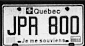
\includegraphics{img/plate.png}
	\caption{Resultat final obtenu à partir de la Figure\ref{grad}\label{plate}}
\end{figure}

\section{Résultats expérimentaux}
Faute d'avoir un jeu de donnée suffisement grand (seulement une trentaine d'image) je n'ai pas pu realiser de statistique. Mais le programme donne de bon résultats dans la majorités des cas.

Cependant il arrive que le programme détecte des "faux positifs" en plus des plaques comme le montre la derniere du Tableau~\ref{result}. Dans la majeur partie des cas ceux-ci seraient très rapidement écarté l'application d'OCR (Optical Character Recognition) chargé de la reconnaissance des caractères de la plaque.

\section{Conclusion}

\begin{table*}[ht]
  \centering
  \begin{tabular}{|m{150pt}|m{150pt}|m{150pt}|}
    \hline
    \multicolumn{3}{|c|}{Reconnaissances effectuées sur des vues de face}\\
    \hline
	  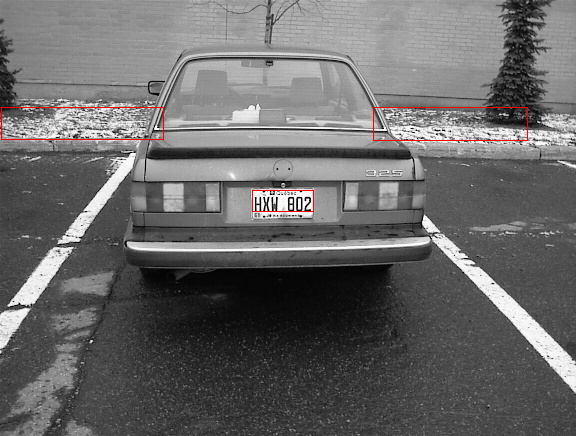
\includegraphics[width=150pt]{img/plate_detect_0.png}&
	  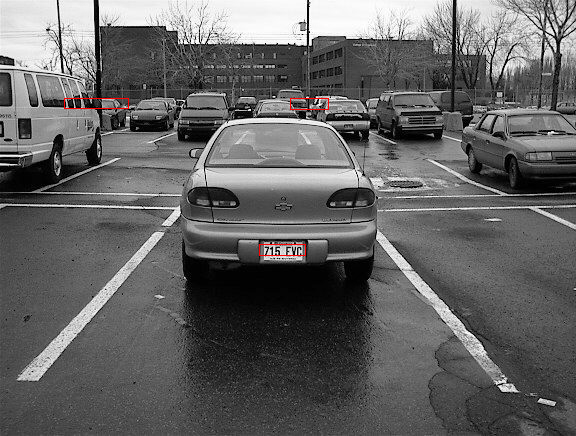
\includegraphics[width=150pt]{img/plate_detect_1.png}&
	  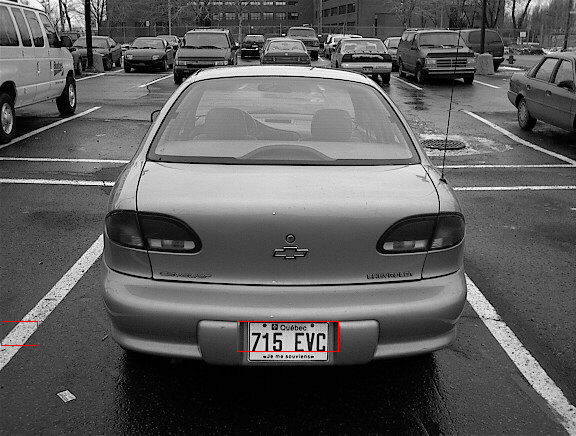
\includegraphics[width=150pt]{img/plate_detect_2.png}\tabularnewline
	  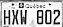
\includegraphics[scale=1]{img/plate_0.png}&
	  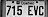
\includegraphics[scale=1]{img/plate_1.png}&
	  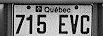
\includegraphics[scale=1]{img/plate_2.png}\tabularnewline
	  \hline
	  \multicolumn{3}{|c|}{Reconnaissances effectées sur des vues latérales}\\
	  \hline
	  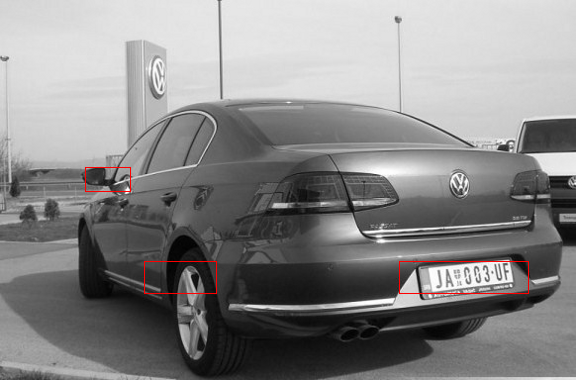
\includegraphics[width=150pt]{img/plate_detect_3.png}&
	  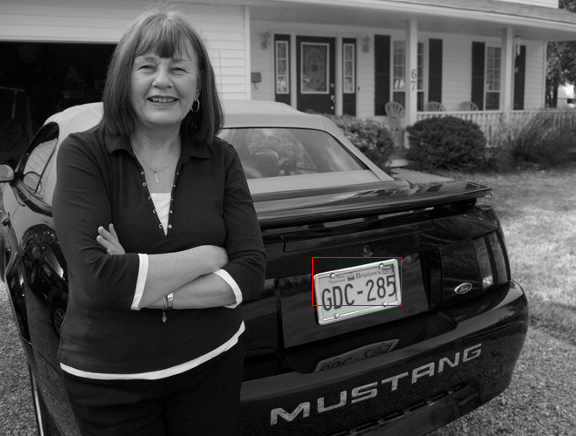
\includegraphics[width=150pt]{img/plate_detect_4.png}&
	  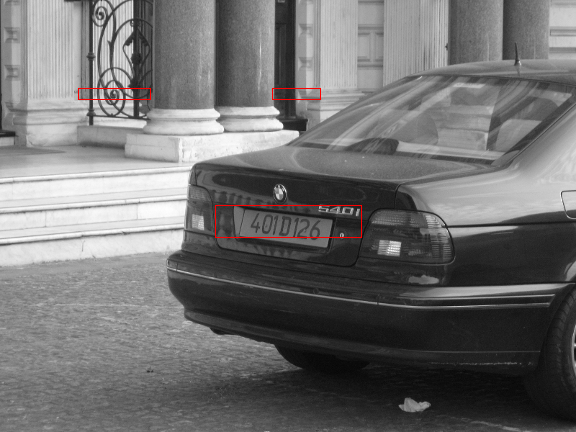
\includegraphics[width=150pt]{img/plate_detect_5.png}\tabularnewline
	  
\includegraphics[scale=1]{img/plate_3.png}&
	  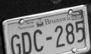
\includegraphics[scale=1]{img/plate_4.png}&
	  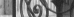
\includegraphics[scale=1]{img/plate_5_0.png} \newline
	  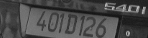
\includegraphics[scale=1]{img/plate_5_1.png}\tabularnewline
	  \hline
	\end{tabular}
	\caption{Resultats expérimentaux\label{result}}
\end{table*}




\begin{thebibliography}{9}
\bibitem{paunwala10}
  \bsc{Chirag N. Paunwala and Suprava Patnaik}, 
  \emph{A Novel Multiple License Plate Extraction Technique for Complex Background in Indian Traffic Conditions}.
  2010.
\bibitem{otsu79}
  \bsc{Nobuyuki Otsu}, 
  \emph{A Threshold Selection Method from Gray-Level Histograms}.
  1979.  

\end{thebibliography}
\end{document}
